\chapter{Event simulation and reconstruction} \label{chp:labelTitle}

An accurate understanding of simulated events and their reconstruction is crucial for a thorough understanding of the collected data. Hence event generators such as $\Madgraph$, $\Pythia$ and $\Herwig$ play the role of hadron colliders and allow some improvement of analyzing power by using an efficient background and signal discriminator.

\section{QCD for hadron colliders} \label{sec::QCDHadron}

The composite nature of protons together with the high-momentum transfers reachable \textit{(conceivable)} at the LHC significantly complicates the event structure. 
For a complete comprehension of the different processes taking place during the generation of a single proton-proton collision the overall algorithm is factorized.
An overview of this factorization is shown in Figure~\ref{fig::EvtShower} for which the different stages are briefly discussed below.

\begin{figure}[htb]
 \centering
 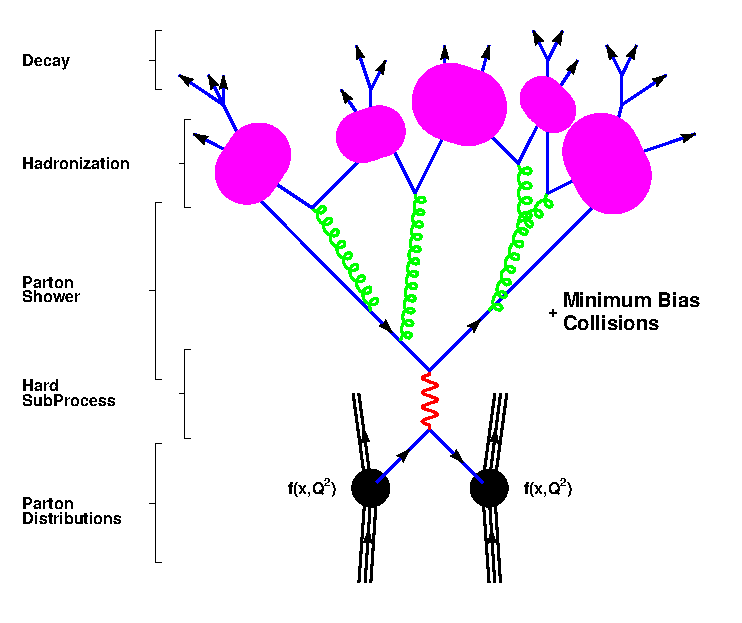
\includegraphics[width = 0.8 \textwidth]{Chapters/Chapter3/Figures/f_shg_event.eps}
 \caption{Schematical overview of the consecutive steps of the event generation process.}  \label{fig::EvtShower}
\end{figure}

\begin{myindentpar}
  \begin{description}
    \item[Parton Distribution Functions] \hfill \\
      In proton-proton collisions both incoming protons can be viewed as a collection of partons whose momentum fraction $x$ within the hadron is parametrized by the so-called parton distribution functions.
    \item[Hard scattering] \hfill \\
      Hard scattering is the perturbative process of two colliding partons, one originating from each proton, that creates high-energetic particles. It can be represented by a factorized product of short-and long-distance contributions as discussed in Section~\ref{sec::HardScattering}.
    \item[Parton shower] \hfill \\
      This phase of the event generation process describes the approximate higher-order corrections induced by emission of additional gluon and/or quarks, as will be explained in Section~\ref{sec::PS}. Depending whether this radiation originates from the incoming or outgoing partons it is denominated, respectively, Initial State Radiation (ISR) or Final State Radiation (FSR).
    \item[Hadronisation] \hfill \\
      The collection of \textit{(receding)} post-shower partons is combined into experimentally observable colour-neutral hadrons as required by colour confinement. This hadronisation process is described by QCD-inspired phenomenological models as discussed in Section~\ref{sec::Hadronisation}.
    %\item[Underlying event (why is this a separate item? Doesn't show up in the schematical overview ...)] \hfill \\
  \end{description}
\end{myindentpar}

The main challenge at hadron colliders \textit{(compared to lepton colliders)} is the missing information about the partons responsible for the hard interaction. 
The event generation process at the LHC is even more arduous due to the QCD activity in a widespread range of involved momentum transfer. %, according to the scale of momentum transfer involved. 
The interaction starts at a scale of barely $1$ $\GeV$ with partons confined in a proton beam, then produces during the hard interaction a few high-energetic outgoing leptons, gauge bosons or partons of which the latter afterwards transform non-perturbatively into final-state hadrons. This large variation in energy range, and corresponding QCD coupling strength, implies that only the event generation's high-momentum transfer contribution can be derived exactly from the QCD Lagrangian while the other aspects have to be expressed using phenomenological non-perturbative models.

\subsection{Hard Scattering} \label{sec::HardScattering}
Most events studied at the LHC involve high-momentum transfers in order to create massive particles or high-energetic jets. The inclusive production cross section of an observable $X$ from hadrons $h_1$ and $h_2$ for these type of interactions can be factorized into:

%Due to the internal structure of the protons, the inclusive cross section $\sigma_{h_{1}h_{2} \rightarrow X}$ cannot be calculated exactly from first principles but has to be factorized in terms of the partonic scattering cross section $\hat{\sigma}_{ab \rightarrow X}$ and the parton distribution functions $f_{a}^{h}$. Therefore, within the collinear limit~\cite{ColLimit}, the inclusive cross section for $X$-production can be written as:
%\\ \textit{Should check whether there is a difference between $\hat{\sigma}_{ab \rightarrow X}$ and $\hat{\sigma}(\Phi_{ab \rightarrow X},\mu^{2}_{F})$??}
\begin{equation} \label{eq::HSXS}
 \sigma_{h_{1}h_{2} \rightarrow X} =\sum_{a,b \in \{q,g\} } \int dx_{a} \int dx_{b} f_{a}^{h_{1}}(x_{a},\mu^{2}_{F}) f_{b}^{h_{2}}(x_{b},\mu^{2}_{F}) \int d\Phi_{ab \rightarrow X} \dfrac{d\hat{\sigma}(\Phi_{ab \rightarrow X},\mu^{2}_{F})}{d\Phi_{ab \rightarrow X}}
\end{equation}
From Equation~(\ref{eq::HSXS}) can be concluded that the hadronic cross section, valid for all orders in perturbation theory, is actually a convolution of a perturbatively short-distance component $\hat{\sigma}_{ab \rightarrow X}$, calculable from Matrix Elements, and an approximately long-distance one, represented by the parton distribution functions (PDF). The PDF $f_{a}^{h}(x_{a},\mu_{F})$ is the probability of encountering parton $a$ with momentum fraction $x_a$ in parent hadron $h$ when this is probed at energy scale $\mu_{F}$. This factorization scale $\mu_{F}$ symbolizes the transition from the short-distance process to the long-distance one (\textit{But this scale is motivated by the soft and collinear divergences which occur whenever a gluon is emitted from a quark so why already introduced in the hard interaction part ?}). 
The partonic scattering cross section $\hat{\sigma}(\Phi_{ab \rightarrow X},\mu^{2}_{F})$ depends on the final state phase space $\Phi_{ab \rightarrow X}$. 
\textit{\textbf{Does this last sentence really add something?}}\\

Equation~(\ref{eq::HSXS}) serves as the starting point for event simulation in general-purpose Monte Carlo event generators which, due to the perturbative nature of the parton-level differential cross section, can be expanded in orders of QCD coupling $\alpha_{S}$. Originally these calculations were performed at leading order (LO), corresponding to $\mathcal{O}(\alpha_{S}^{2})$, however this only describes the simplest processes taking place in hadron colliders and does not correspond to reality where additional radiation on top of $X$ occurs. Moreover the current theoretical precision for QCD requires at least next-to-leading order (NLO) calculations. Hence much effort has been devoted in order to overcome the infrared singularities in QCD allowing to extend the matrix element generators to perform these NLO calculations in an automated way and thereby (?) significantly improving accuracy and predictive power.\\

\textit{\textbf{Rewrite this part once is known which generators are actually used and which not at all ...\\}}
Many different event generators exist, but not all seem to be actually used for MC samples used in this thesis...\\
Herwig and Pythia are two general-purpose event generators, but they are both lacking NLO information. Only way to acquire NLO calculations is by incorporating full NLO corrections in the parton shower using the Powheg formalism. Sherpa is another event generator which has NLO information but does not seem to be used (so no need to discuss).\\
The more widely used event generators incorporate NLO corrections in the hard interaction: MadGraph/MadEvent, MC@NLO and Powheg.

\begin{myindentpar}
  \begin{description}
    \item[MadGraph/MadEvent] \hfill \\
      MadGraph is a matrix element generator for decays and $2$ $\rightarrow$ $n$ scatterings. \textit{(Not very clear, is it now NLO or is it tree-level ... ?)}
    \item[Powheg and MC@NLO] \hfill \\
      Powheg and MC@NLO are two event generators which are capable of calculating NLO corrections and, even more important, correctly matching them with the additional particles created during the parton shower step, which will be discussed in detail in \ref{sec::PS}
  \end{description}
\end{myindentpar}

\textit{What else can/should be written about this subject ...?}\\
\textit{Maybe brief discussion about LHAPDF and the used PDF set in this thesis (or does this only come after the Parton Shower part has been explained?)}

\subsection{Parton shower} \label{sec::PS}

The hard interaction does a great job in describing the primary collision between the two initial partons using the lowest order matrix-elements. However this process is lacking information about \textit{(the internal structure of jet and)} the non-perturbative confinement of partons into colour-neutral hadrons at low energy scales. This iterative process of higher-order emission corrections is defined by the Parton Shower (PS) formalism.

The partons formed during the hard scattering are prone to gluon radiation emission, $q$ $\rightarrow$ $qg$, and gluon branching, $g$ $\rightarrow$ $gg$. The first type of parton branching corresponds to Brehmstrahlung in QED while the second one has no analogy in QED and is caused/provoked by QCD's non-abelian nature. Both processes are incorporated in the PS formalism which sequentially lowers the transverse momentum of the contributing partons until the QCD confinement limit is reached, resulting in a broad parton cascade.
\\

The parton shower formalism's objective is to convert the inclusive cross section for the production of parton $a$ into the exclusive cross section taking into account a number of additional less-energetic particles.
%represent the large number of final state partons as a primary hard interaction surrounded with (chains of parton branchings) showers. 
Hence the complex $2$ $\rightarrow$ $n$ process will be decomposed into a hard interaction with momentum transfer $Q$ and a succession of gluon radiations each with momentum transfer $Q_{i}$; a justifiable approach in the approximation $Q_{i}^{2}$ $\ll$ $Q^2$ which is defined as the collinear\footnote{Two particles are collinear in case they are close in angle.} limit. 
%\textit{The exclusive cross section of the overall process can be associated with the cross section of the hard interaction but incorporates minor deviations to take into account the reduced energy available for the hard scattering due to the initial state radiation. \textbf{Really useful this XS info?}}
The Alterelli-Parisi splitting functions, denoted $P_{ba}(z)$, describe this collinear splitting of parton $b$ into parton $a$ and are defined as~\cite{}:
%The collinear splitting of parton $b$ into parton $a$ is described by the Alterelli-Parisi splitting functions $\hat{P}_{ba}(z)$, defined as~\cite{}:
\begin{eqnarray}
 & P_{qq}(z) = \dfrac{4}{3} \dfrac{1+z^{2}}{1-z}    & P_{qg}(z) = \dfrac{4}{3} \frac{1+(1-z)^{2}}{z} \\
 & P_{gq}(z) = \dfrac{n_{f}}{2} (z^{2} + (1-z)^{2}) & P_{gg}(z) = 3 \dfrac{z^{4}+1+(1-z)^{4}}{z(1-z)}
\end{eqnarray}
where $n_{f}$ represents the number of quark flavours.
\\
These splitting functions are divergent in the case of $z$ $\rightarrow$ $1$, corresponding to soft gluon emission as $z$ is the momentum fraction carried away by the parton $a$. 
Since reality is known to be finite these soft divergences, together with the collinear divergencies ($\theta$ $\rightarrow$ $0$), have to be excluded by introducing a cutoff scale on the transverse momentum $k_{t}$ ($\simeq$ $E\theta$ \textit{relevant?}) below which all remaining perturbative effects are absorbed by the parton distribution functions. 
The freedom of choosing this factorization scale $\mu_{F}$, generally around $1$ $\GeV$, necessitates the introduction of the DGLAP (Dokshitzer-Gribov-Lipatov-Altarelli-Parisi) evolution equations~\cite{}, which represent the fact that any parton $a$ may have been produced by the branching of parton $b$ at slightly higher scale $\mu_{F}^2 + d\mu_{F}^2$:\\
\begin{equation}\label{eq::PSProb_NoSudakov}
 \mu_{F}^2 \dfrac{d f_{a}^{h}(x,\mu_{F}^{2})}{d \mu_{F}^{2}} = \sum_{b \in \{q,g\} } \int_{x}^{z_{max}} \dfrac{dz}{z} \dfrac{\alpha_{S}}{2 \pi} P_{ba}(z) f_{b}^{h}(x/z, \mu_{F}^{2})
\end{equation}
Even though the introduction of the factorization scale resolved the divergencies, the branching probability in Equation~(\ref{eq::PSProb_NoSudakov}) can still exceed unity. This because also the virtual divergencies which lead to cancelations have been removed by this cutoff. Hence total conservation of probability should be restored by adding an additional term to the DGLAP equations:
\begin{eqnarray}
 \mu_{F}^2 \dfrac{d f_{a}^{h}(x,\mu_{F}^{2})}{d \mu_{F}^{2}} & = & \sum_{b \in \{q,g\} } \int_{x}^{z_{max}} \dfrac{dz}{z} \dfrac{\alpha_{S}}{2 \pi} P_{ba}(z) f_{b}^{h}(x/z, \mu_{F}^{2}) \nonumber \\
                                                             &   & - f_{a}(x,\mu_{F}^{2}) \sum_{b \in \{q,g\}} \int_{z_{min}}^{z_{max}} dz \dfrac{\alpha_{S}}{2 \pi} \dfrac{1}{2} P_{ab}(z)
\end{eqnarray}
The above equation can be further simplified by identifying the Sudakov form factor, which represents the probability for a parton not to undergo a branching between the energy scales $t^{'}$ and $t$.
\begin{equation}
 \Delta_{a}(t,t^{'}) = \exp \left\lbrace - \sum_{b \in \{q,g\}} \int_{t}^{t^{'}} \dfrac{dk_{T}^{2}}{k_{T}^{2}} \int_{z_{min}}^{z_{max}} dz \dfrac{\alpha_{S}}{2 \pi} \dfrac{1}{2} P_{ab}(z) \right\rbrace
\end{equation}
Now the basic building block of the parton shower algorithm, the probability distribution for one emission to be accompanied by a parton with momentum fraction $z$, that will be iterated over during the shower process can be summarized as:
\begin{equation}
 \dfrac{d}{d \log \mu_{F}^{2}} \log \dfrac{f_{a}(x,\mu_{F}^{2})}{\Delta_{a}(t_{c},t)} = \sum_{b \in \{q,g\}} \int_{x}^{z_{max}} \dfrac{dz}{z} P_{ba}(z) \dfrac{f_{b}(x/z,\mu_{F}^{2})}{f_{a}(x,\mu_{F}^{2})}
\end{equation}
\textit{\textbf{Is this transformation between t and $\mu_{F}^{2}$ completely correct ??  How to set $t_c$ in this $\Delta$ term .. ? Formula's taken from ``Introduction to PS event generators''!}}\\
%\\
%\textit{$P_{ba}$ can be easily translated to $P_{b \rightarrow a+c}$ by applying the allowed emissions.\\
%qq corresponds to q $\rightarrow$ q which can only be accompanied by gluon radiation hence $P_{qq}$ = $P_{q \rightarrow q g}$ in the definition used above. (check papers for rest)}\\

The parton shower algorithm outlined above is applicable for both initial and final state radiation since their branching probabilities are similar. However the actual implementation in the Monte Carlo event generators is performed in an entirely different manner. 
Initial state radiation is simulated by employing a backward evolution: the Monte Carlo event generator starts from the desired hard interaction and surrounds the initial partons with additional radiation only afterwards. This because each parton branching significantly reduces the energy of the initial partons and therefore the possibility to produce the hard process of interest, such as top-quark pair production. 
%In order to avoid the generation of billions of events and keeping only a couple relevant ones, the Monte Carlo event generators employ a backward method. 
Final state radiation on the other hand is taken into account in a much more straightforward way: the parton branching starts at the hard interaction scale $Q^{2}$ and is sequentially lowered until the factorization scale $\mu_{F}^{2}$ is reached.

\subsubsection{Combine hard scattering with parton showering}
From the overview given above can be understood that the Matrix-Element and Parton-Shower algorithm have some crucial differences in how to simulate $X+n$-jet topologies.
The former one reliably describes the simulation of well separated hard partons but lacks information about the collinear and soft partons while for the latter one this is exactly the contrary. Hence for accurately describing the entire event simulation chain up to the final-state hadrons both approaches should be combined. However this is not a straightforward process since possible double-counting can occur since a hard parton of a $X+2$-jet event can originate either from a $X+2$-jet fixed-order matrix-element calculation or from a hard emission during the showering of the $X+1$-jet event.
\\

Different approaches exist for correctly dealing with this double-counting issue and the ones used in this thesis are outlined below. A distinction should be made whether the matrix-element calculations have been performed at LO or NLO accuracy since the latter significantly complicates the combination procedure.\\
In case LO matrix-elements have to be combined with the parton shower the MLM approach is applied which imposes a cut on the jet transverse momentum to ensure any hard jet in the event to originate from the hard interaction. So an event is rejected in case more than the requested number of jets have transverse momentum above the merging scale. The hard jets produced in this way are certain to be described by tree-level matrix elements since the merging scale is chosen to be larger or equal than the matrix-element cutoff scale.
As in the parton shower algorithm, this approach can be depicted by introducing Sudakov factors that represent the probability for not undergoing a hard scattering below the merging scale during the showering process.
The MLM approach is used in $\Herwig$ and $\Pythia$ (\textbf{when used?}) and results in a parton shower structure with LO accuracy which is applied in a broad range of LHC analyses.
\\
Even though the LO results using the MLM approach are successful in describing shapes of experimental distributions considerable gain can be reached by extending to NLO accuracy. 
%\textit{Such a matching aims to, beside the real corrections which are included in the LO process as well, include the virtual corrections correctly (\textit{useful??})} 
The main challenge of matching NLO calculations with parton showers is to overcome the additional double-counting introduced by the approximate NLO corrections included in the parton shower generators. 
One of the first acceptable NLO matching methods which correctly tackles this double-counting issue was the so-called $MC@NLO$ algorithm, which only applies the parton-shower algorithm on PS-corrected NLO matrix-elements.
The correction term is obtained by first computing the NLO matrix-element corrections to $n$-body decay, then calculating how the first shower of a $n$-body decay would populate the $n+1$-body phase space and finally subtracting this approximate shower calculation from the exact NLO matrix-element. The downside of the $MC@NLO$ approach is two-fold: the subtraction of the two contributions can lead to negative weights and the subtraction terms are generator-dependent such that for now only $\Herwig$ can be used for performing the parton shower. 
\\
Hence a new NLO matching method was developed to overcome both the presence of negative weights and the generator-dependency of the $MC@NLO$ approach. The $Powheg$ approach starts from the hardest emission using full NLO accuracy and applies normal showering afterwards. This implies that only one emission beyond LO should be generated in order to obtain NLO accuracy. In this thesis the $Powheg$ approach is combined with the $\Pythia$ parton shower algorithm.

\subsection{Hadronisation} \label{sec::Hadronisation}
The missing link in the event generation process is how the quarks and gluons produced during both the hard interaction and the showering turn into experimentally observable colour-neutral hadrons. This step is defined as the hadronisation or fragmentation process and is represented by phenomenological models since it cannot be calculated from first principles due to the corresponding low energy scales.
Two distinct models for describing this non-perturbative process are used today: the Lund string model~\cite{Lund} and the cluster model~\cite{ClusterModel}. The former one is implemented in $\Pythia$ while the latter one is used by $\Herwig$.
\\
The Lund string model is based on linear confinement, which states that the potential $V$ between a quark-antiquark increases with separation distance $r$ due to the presence of a strong QCD colour field: %, as depicted in Equation~(\ref{eq::VQCD}).
\begin{equation}\label{eq::VQCD}
 V = \kappa r ~~~ \kappa \sim 1 \dfrac{\GeV}{fm}
\end{equation}
Hence the kinetic energy of such a parton pair will transform into potential energy and accumulate while receding. 
Once sufficient energy is stored in the colour string stretched between the quark $q$ and anti-quark $\bar{q}$, the string will split into a new $q\bar{q}$ pair with a colour string surrounding each parton pair.
A fraction of the potential energy will be absorbed by the parton creation and, as a consequence, lowering the remaining energy during each following string splitting until no subsequent splittings can occur.
The probability for the creation of a quark with mass $m$ and transverse momentum $\pT$ during such a splitting is given by:
\begin{equation}\label{eq::mBot}
 %\exp \left( -\frac{\pi m^{2}_{\bot}}{\kappa} \right) =
 \exp \left( -\frac{\pi m^{2}}{\kappa} \right) \exp \left(-\frac{\pi \pT^{2}}{\kappa} \right)
\end{equation}
However, the above formula only represents the formation of light $u$-, $d$- and $s$-quarks since the presence of the mass term implies that the production of heavier quarks is suppressed during this step of the event generation process. 
%Heavier mesons are only created afterwards when the unstable light mesons decay further into stable final-state hadrons.
%The Lund string model is also valid for baryon creation, which in it simplest form is obtained by allowing antidiquark-diquark production during string breaks.
\\
%The quantity $m^{2}_{\bot}$ $=$ $m^{2} + p_{x}^{2} + p_{y}^{2}$ in Equation (\ref{eq::mBot}) is the transverse mass 
The transition of these free quarks into bound states is described by the Lund fragmentation function which gives the probability of a colour string to produce a hadron $h$ with mass $m_{h}$, transverse momentum $p_{T}$ and longitudinal momentum fraction $z$ during the string-breaking process. The fragmentation function exhibits a ``left-right'' symmetry since the splitting sequence should be identical whether is started from the quark or anti-quark.
\begin{equation}
 f(z) \propto \frac{1}{z} (1-z)^{a} \exp \left( - \frac{b(m_{h}^{2} + p_{\rm T,h}^{2})}{z} \right)
\end{equation}
with $a$ and $b$ free parameters of the model.
In order to overcome the suppression of heavier hadrons an additional $1/z^{bm_{Q}^{2}}$~\cite{} factor has to be taken into account.
\\
The second hadronisation model, the cluster model, is based on the preconfinement property of QCD and splits the gluons non-perturbatively into $q\bar{q}$ pairs after the parton shower. From this clusters, or colour singlet combinations of partons, can be created which transform into hadrons either directly or through splitting processes depending on their mass. 
%~\footnote{This implies that colour singlet combinations of partons (= clusters) can be formed with an asymptotically universal invariant mass distribution \textit{NOT OWN WORDS}}. At the end of the parton shower gluons are splitted into $q\bar{q}$ pairs and colour-connected pairs give rise to clusters from which hadrons are formed. 
\textit{More detail needed on this second model ?}
\\
\textit{Something about decay of unstable particles?}

\subsection{Additional event activity (find good title)}% and Multiple Parton Interactions (?)}

The previous sections have provided a detailed overview of the event generation process from start to finish, but were limited to the ideal situation where only one parton present in each parton contributes to the production of final-state hadrons. A more realistic representation would be to take into account the additional activity which occurs in coincidence with the primary parton collision. 
\\

The term Underlying Event (UE) has been adopted as collective noun to depict the types of additional interactions during a single hadron-hadron collision that could possibly alter the final-state. At the LHC where protons are used as incoming particles, two distinct soft phenomena contribute to the UE: the beam remnants and the multiple parton interactions (MPI).
The beam remnant is defined as the remainder of the proton after the hard-interacting partons are extracted. The non-zero colour charge of the beam remnant implies the creation of additional hadrons during the hadronisation process.
Multiple parton interactions represent the distinct scattering processes that could take place between other incoming partons. 
The presence of MPI can be understood from the composite nature of protons implying that each parton is as likely to undergo scattering interactions within one single hadron-hadron interaction.
The jets produced from the MPI  are in general less energetic than the principal hard interaction and the chances of producing an extra hard interaction during this process are very rare.
As a result the underlying event is mainly saturated with low-energetic partons which tend to travel along the beamline such that it can be studied by selecting a specific topological structure.
%tend to travel along the beamline, allowing the possibility to study the underlying event in more detail. The chances of producing an additional hard interaction 
\\
The complexity of the underlying event lies in the fact that it involves both non-perturbative and perturbative QCD making it, at least for the moment, practically impossible to understand the physics. Hence Monte Carlo models have to be tuned; i.e.\ constraining free parameters using existing data; in order to accurately describe the collider physics.
\\
\textit{Necessary to explain the specific methods used by Pythia and Herwig?}
\\
%As mentioned before, the exchanged QCD particles have colour charge implying that even a limited number of soft particles produced in this underlying event can have a major influence on the particle multiplicity in the final state. 
%\textit{Mention something about the consequences ...}
%In 1987, Sj\"ostrand and van Zijl proposed a first detailed Monte Carlo model for perturbative MPI, which is still considered as the basis for modern implementations~\cite{SjostrandAndZijl} (Check reference 76 of QCD for Collider Physics). \textit{Is this model-part necessary?}\\
\textit{Should check whether UE is one of the important systematics or not... This determines in how much detail this section should be explained!}
\\

Another important contribution to additional event activity which significantly complicates the final-state topology of hadron-hadron collisions is pileup (PU) or additional hadron-hadron collisions. These type of interactions occur because hadron-hadron collisions are not performed between two single hadrons but between bunches of hadrons. Therefore it is again likely for multiple hadrons to result in a hard interactions surrounded with UE during one bunch crossing. A distinction can be made whether the PU originates from the same bunch crossing as the hard interaction or from a previous bunch crossing, which are defined as in-time PU and out-of-time PU, respectively. The latter one can manifest itself when the bunches are spaced such that the next one arrives before the previous one evacuated completely from the detector.

\section{Simulating detector response} \label{sec::DetectorSim} %Detector simulation (CHANGE TITLE!)}
The Monte Carlo event generators adopt an approach independent of the considered accelerator complex, besides starting with the correct incoming partons, and can thus be applied in a very broad physics range. In order to study specifically proton-proton collisions collected at the CMS detector, the simulated events are pushed through a dedicated detector simulation chain based on the $\Geant$ software toolkit~\cite{}. This software package contains a full geometrical description of the CMS detector and a detailed mapping of the magnetic field, implemented in a flexible way allowing the activation and deactivation of specific detector subsystems.
\\
This detailed detector simulation treats the simulated events as actual data originating from the interaction point and propagates them through the entire detector while taking into account energy loss caused by interactions with the detector material. 
The simulated energy deposits in the different subsystems are converted into electronic signals based on the actual detector behavior resulting in a completely identical treatment as for real data.
During this step pileup is included by overlaying the primary interaction with generated proton-proton events simulated in an identical manner. 
The mixing procedure applied depends on the specific subdetector considered, especially for incorporating out-of-time pileup since different numbers of preceding and succeeding bunch crossings should be regarded.
Employing the full simulation chain results in very good agreement with actual data and is therefore widely used in many physics analyses, including this thesis. However this full simulation or FullSim is very time-consuming, in general several minutes are necessary for processing a single event, resulting in the development of a fast simulation chain, denominated as FastSim. 
The simplified geometry adopted in the FastSim approach reduces the CPU-time with roughly a factor $100$.
\textit{Is FastSim somewhere used in my thesis?}\\
An overview of the Monte Carlo samples used in this thesis are listed in Table~\ref{table::Samples}.

\begin{table}[h!t]
 \caption{Title above for tables.} \label{table::Samples}
 \centering
 \begin{tabular}{|c|c|}
  \hline
  Sample & Generator \\
  blabla & blabla \\
  \hline
 \end{tabular}
\end{table}

\section{Physics object reconstruction (CHANGE TITLE!)} \label{sec::PhysicsObjects}

\textit{Important to first explain the separate construction of both the muon and electron candidates because they are actually used as a starting point for the PF algorithm. The PF algorithm should not be seen as something completely disconnected because was actually added on top of the already existing reconstruction methods in order to improve the efficiency and reduce the corresponding fake rates.}

\subsection{Muon reconstruction}\label{subsec::Muon}

The muon reconstruction algorithm is designed such to fully exploit the excellent reconstruction efficiency in both the tracker and the muon system.
%Since the muon traverses the entire tracker detector without siginificant energy loss it will produce detectable hits in multiple layers of the tracking system. 
Hence tracks reconstructed in the inner tracker and the muon system separately are combined into actual muon candidates. In order to distinguish these two types of muon-seeds they are called \textit{tracker track} and \textit{standalone-muon track}, respectively.
\\
The identification of standalone-muon tracks is performed in two consecutive steps. First local reconstruction starts by constructing track segments from the detected hits in the DT and/or CSC chambers. Afterwards the track segments found in the innermost chambers are used as seeds for the standard reconstruction algorithm based on the Kalman Filter technique, as discussed in Section \ref{sec::KFTracking}. First an inside-out Kalman Filter is applied which\footnote{ (takes into account the muon energy loss in the material, the effect of multiple scattering and the non-uniform magnetic field. -- or is this general the case for a KF?) This procedure} propagates the muon track to the next layer, compares with the measured energy deposits and updates the track parameters accordingly. Once the most outer layer of the muon system is reached, a second Kalman Filter is used to calculate the track parameters at the most inner muon station. Finally, in order to improve the momentum resolution, an additional beamspot constraint is applied to the track parameters before identifying the standalone-muon track.

Proper muon candidates combining information from both the tracker detector and muon system can be obtained using two different methods. In case the muon identification starts from the standalone-muon tracks so-called \textit{global muons} are reconstructed while the collection of tracker tracks gives rise to \textit{tracker muons}.
The global muon candidates are reconstructed by identifying a matching tracker track, for each standalone-muon track, by propagating both track parameters onto a common surface. Then for each pair the hits are combined into a global-muon track using an outside-in Kalman Filter Technique. The identificitation of muon candidates as global muons is especially powerful when a high quality muon track was found in the muon detector. However in some cases it can occur that the standalone-muon reconstruction fails because of a lack of hits. This is most likely to happen in the presence of low transverse momentum muons which are unable to deposit sufficient energy deposits in the muon spectrometer. Hence for these muons the tracker-muon reconstruction is very useful since it extrapolates all tracker tracks with transverse momentum $\pT$ $>$ $0.5$ $\GeV$ and total momentum $p$ $>$ $2.5$ $\GeV$ to the muon system. If at least one muon segment corresponds with the extrapolated track, the tracker track fullfilled the tracker muon requirements and is identified as such.
\\
Since both approaches have specific benefits they are combined in order to have a robust and highly efficient (\textbf{How much?}) muon reconstruction (\textit{throughout all energy ranges}).
\\
\textit{Something about charge identification necessary?}
 
\subsection{Electron reconstruction} \label{subsec::Electron}

The thickness of the CMS tracker requires a dedicated elektron-track reconstruction such to correctly incorporate the energy loss caused by Brehmsstrahlung. 
This photon radiation significantly lowers and smears the initial momentum of the electron, predominantly along the $\phi$ direction, resulting in a more complex and less straightforward electron reconstruction algorithm.
Hence in stead of applying the general Kalman Filter track reconstruction approach, a dedicated electron-reconstruction algorithm based on a Gausian Sum Filter (GSF) fit is developed. The main benefit of the GSF algorithm is the possibility to model changes in curvature radius throughout the different tracker layers. 
Unfortunately the GSF fit is rather CPU intensive and is therefore only be applied on a subset of track seeds defined as electron seeds.
%Since the electrons traverse a (vast) amount of matter before reaching the electromagnetic calorimeter where they can deposit their energy, Brehmsstrahlung will occur. 
%As a consequence the electron reconstruction algorithm is more complex and less straightforward than the previously discussed muon reconstruction algorithm.%, however, the main idea still comes down to associating a charged-particle track with an ECAL cluster.

The identification of the subset of electrons seeds relevant for the electron-track reconstruction can be performed by two different seeding algorithms: an ECAL-based or tracker-based algorithm.
The ECAL-based approach starts from the energy deposits recovered in the electromagnetic calorimeter and extrapolates them back to the interaction vertex. In order to take into account the Brehmsstrahlung effects, the cluster is enlarged into a so-called supercluster and the extrapolation to the tracker is performed from the energy-weighted average position of this supercluster. The tracker seeds corresponding with hits of the extrapolated supercluster are then defined as electron seeds. The tracker-based approach on the contrary starts from charged-particle tracks reconstructed with the general KF reconstruction algorithm. The tracker seeds are in this case obtained using an MVA method in order to only select the ones compatible with the electron-particle hypothesis.

After the tracker seeds have been identified, the specific electron-track fitting procedure can be applied. As mentioned above, this is done by a Gaussian Sum Filter fit which describes the energy loss in each tracker layer by a mixture of Gaussian distributions. Such a representation is advisable in the presence of Brehmsstrahlung since the normal Kalman Filter fit only assumes a single Gaussian energy loss distribution for a particle traversing the detector. The track fitting provides electron-tracks up to the electromagnetic calorimeter such that the corresponding track parameters can be obtained at the ECAL surface allowing the estimation of the energy loss due to Brehmsstrahlung.

The GSF tracks recovered with this dedicated electron reconstruction algorithm are afterwards translated into actual electron candidates in two different ways: either based on a track-cluster association criterion or by the PF event reconstruction algorithm. The former one, which depens on the seeding method used, will be discussed here while the PF-approach will be discussed in Section \ref{subsec::PF}.
In case the ECAL-based seeding algorithm is used for identifying the electron seeds, the electron track is associated with the supercluster used for the seed reconstruct based on a geometrical matching. For the tracker-based seeding algorithm the association is done with a PF cluster based on a MVA combining information on track observables and electron PF cluster observables. \textit{So how is dealt with the photon ECAL deposits in this case?} 

\subsection{The Particle-Flow event reconstruction algorithm} \label{subsec::PF}

In order to reconstruct the direction, energy and type of all stable particles as accurately as possible the particle-flow (PF) algorithm combines the information of the different CMS subdetectors. The obtained collection of individual particles is then used to reconstruct jets and determine missing transverse energy.
The main benefit of the PF approach is the large gain in efficiency by combining less precise subdetectors with more granular ones.
\\
The PF algorithm uses a stepwize approach \cite{}, starting by identifying fundamental elements such as charged-particle tracks, calorimeter clusters and muon tracks. Then the algorithm links these distinct building bricks of the different subdetectors topologically such to construct specific building blocks. As a final step the building blocks are converted into stable particles.
%(\textit{This approach exploits the high granularity of the ECAL and the very precise tracker immersed in a uniform axial magnetic field of 3.8 T.})

\subsubsection*{Reconstructing and combining the fundamental elements}

The building bricks used by the PF event reconstruction algorithm have to be measured with very high efficiency and a low fake rate because most of the stable particles have rather low momentum, even in very energetic collisions.
The dedicated identification algorithms developed for the different subdetector bricks are optimized such to effectively deal with this demanding environment.
\\
The iterative tracking algorithm used to reconstruct charged-particle tracks fullfills both requirements with flying colours. The CMS tracking detector can be considered the cornerstone of the PF event reconstruction since it measures the momentum of charged hadrons with a higher resolution than the calorimeters and even provides a precise determination of the charged-particle direction at the production vertex before any influence from the magnetic field. The iterative tracking algorithm starts from very tight charged-particle seeds and progressively loosens the track seeding criteria. At each iteration hits assigned to the tracks found during the previous iteration are removed (\textit{What is this part doing?})
\\
The calorimeter clusters are reconstructed in a high efficient and low fake rate manner using a clustering algorithm specifically developed for the PF event reconstruction. In this algorithm the seeds are defined as calorimeter cells with energy above a certain threshold. These cluster seeds are then transformed into so-called topological clusters by accumulating calorimeter cells adjacent to the cells present in the cluster. In order to suppress electronics noise the calorimeter cells are required to exceed a given energy threshold. Finally each topological cluster results in several particle-flow clusters: as much as cluster seeds present in the topological cluster.
\\

Since each particle is expected to give rise to multiple building bricks a non ambiguous linking algorithm that excludes any possible double-counting is applied. This algorithm connects elements presumed to correspond to the same particle and quantifies the quality of the linkage by the distance between the considered elements. For example a charged-particle track is linked with a PF calorimeter cluster if its extrapolated position lies within the cluster boundaries. This specific linking is also performed between charged-particle tracks and ECAL clusters in order to take into account the energy deposited by Bremsstrahlung photons emitted by electrons. Because the above explained clustering algorithm is performed separately in each of the calorimeter sub-detectors linking between different calorimeter clusters is also considered. In this case a linkage is established when the cluster position of the more granular calorimeter is within the cluster envelope of the less granular one. Finally the linking algorithm matches charged-particle tracks and muon tracks based on a global $\chi^{2}$ track fit in order to create so-called global muons. \textit{Is this really part of the PF algorithm, this is the Global Muon reconstruction ...}
\\
\textit{Nothing specific about muon tracks??}

\subsubsection*{Identifying stable particles}
After establishing the fundamental elements and the linkages amongst them, the collection of stable particles is reconstructed by the particle-flow algorithm. This occurs in a gradual manner, first the PF muons and PF electrons are identified and from the remaining elements the charged hadrons, photons and neutral hadrons are distinghuised.
\\
The global and tracker muons (, as reconstructed in Section \ref{subsec::Muon},) can only be promoted to PF muons once the contamination from misidentified charged hadrons is removed.
Both contributions can be distinguished based on different criteria, such that three specific selection procedures are applied.
At first the so-called isolated selection is applied, which considers only global muons and has the loosest selection of all three (\textit{since almost no additional neutral particles are expected to lie within their vicinity -- explain what it does ...(charged hadrons will not be isolated right?}). 
The remaining muon candidates are passed to the PF-loose and PF-tight selection, which are developed such to identify muons within jets. The PF-tight selection aims to reject \textbf{hadronic punch-through\footnote{Defined as hadron shower remnants penetrating through the calorimeters and reaching the muon system.} (?)} by combining information from the muon system and the calorimeters while the PF-loose selection tries to recover muon candidates that have a track momentum significantly larger than the corresponding calorimeter deposit, a combination incompatible with the charged hadron hypothesis.
\\
The reconstruction of PF electrons starts from the GSF track (, see section \ref{subsec::Muon}) for which the outermost track layer position is extrapolated to the ECAl and associated with the closest PF cluster, this to incorporate possible curvature alterations by Brehmsstrahlung.
Afterwards the energy of the corresponding photon clusters are assigned to the total electron energy. Finally the electron candidates are distinghuised from charged hadrons using a multivariate analysis based on variables related to energy and geometrical matching between the track and the cluster, two purely calorimeter-based variables and several genuine tracking quantities.

After the identification of the PF muon and PF electron candidates the remaining charged-particles tracks and PF calorimter clusters are translated into charged hadrons, photons or neutral hadrons.
Whenever a linkage can be performed between a particle track and a calorimeter cluster with compatible energy measurements, it is defined as a charged hadron candidate. In case the calorimeter measurement is larger the excess is assigned to a photon or a neutral hadron depending whether the cluster is found within the ECAL or HCAL, respectively.
The collection of remaining calorimeter clusters unable to be linked with a charged particle track are also identified as photons or neutral hadrons.
%\textit{extensive enough?}

\subsection{Jet reconstruction}
The reconstruction of jets is less straightforward than the other physics objects explained before because they should be seen as a collection of hadronic activity combined into a single cone. However the event topology of interest, $t\bar{t}$ $\rightarrow$ $bjjbl\nu_{l}$, contains four jets so reconstructing this object in a correct and accurate way is very important.
\\
\textit{Where find more information?}
 
\subsubsection*{Jet clustering algorithm}
Many different jet clustering algorithms exist but in this thesis only the cluster-based ones will be used and hence explained. This type of jet clustering algorithms starts from a collection of stable partons and calorimeter cells and combines them into a cone with radius $R$ \textit{(Is this really correct? --  can also use 'into a jet')}. This clustering procedure uses a distance-based approach since it looks for each object $i$ whether another object $j$ can be found within the predefined cone radius $R$ taking into account the transverse momentum $k_{\bot}$ of both objects.
\\
The distance measures used in this jet clustering algorithm are given in Equations (\ref{eq::JetClustering1}) and (\ref{eq::JetClustering2}) where the first one defines the distance between the two objects while the second one represents the distance between the object $i$ and the beam (B). Here $\Delta_{ij}^{2}$ $=$ $(y_i - y_j)^{2} + (\phi_i - \phi_j)^2$, the $(y,\phi)$ distance between both objects and $p$ can be intepreted as a parameter which controls the relative power between the energy and the geometrical scales.
\\
\begin{eqnarray}
 d_{ij} & = & \min(k_{\bot i}^{2p}, k_{\bot j}^{2p}) \frac{\Delta_{ij}^{2}}{R^{2}} \label{eq::JetClustering1} \\
 d_{iB} & = & k_{\bot i}^{2p}                                                      \label{eq::JetClustering2}
\end{eqnarray}
The value given to the parameter $p$ defined in the two distance definitions, which governs the relative power of $k_{\bot}$ versus $\Delta_{ij}^{2}$, results in different cluster-based jet algorithms; two of which are used in this thesis. When this parameter takes the value $1$ the $k_{\bot}$ algorithm can be retrieved, which is used in ... (used?) . 
In the case of $p$ $=$ $-1$ the jet algorithm is defined as the anti-$k_{\bot}$ algorithm. This algorithm is used for ... (\textit{\textcolor{red}{How to know where which algorithm is used??}})
Within this jet clustering algorithm soft particles prefer/tend to cluster with hard particles (in stead of with other soft particles) implying robust jet boundaries with respect to soft radiation. Both jet clustering algorithms are infrared and collinear safe, meaning that the created jet collection is not sensitive to soft emission and collinear splitting, respectively.
\\

The jet clustering algorithm creates jets by looking for the smallest of these distances. Whenever the distance $d_{ij}$ is smallest, the objects $i$ and $j$ are merged into a single object and stored as such in the list. However, in case the distance $d_{iB}$ is smallest, the object $i$ is removed from the list of input objects and categorized as a final jet. Afterwards the distances are recalculated and this procedure continues until no input objects remain.
\\
The merging of two different objects into a single one is done using one of the existing recombination scheme, in the case of this thesis the E recombination scheme is used. This scheme calculates the four-momentum of the new object by simply adding the four-momentum of its constituents. (\textit{What about eta and phi?? -- explanation about ET scheme needed as well?})

\subsubsection*{Jet energy calibration}

Idea of jet energy calibration is to relate, on average, the energy measured for the detector jet to the energy of the corresponding true particle jet (\textit{\textbf{Line taken EXACTLY from 1107.4277 page 8}})\\
Important point is that this takes place in a factorized approach where each subsequent correction term is applied on transverse momentum corrected with all previous correction terms.

\begin{myindentpar}
  \begin{description}
    \item[L1 pileup offset correction] \hfill \\
    The first contribution\footnote{Is applied on the ``remainder of diffiuse energy'' after the Charged Hadron Subtraction (CHS)} to the factorized correction chain aims to remove the additional energy deposits originating from pileup interactions in order to remain with a only the high-$\pT$ scattering. The corresponding correction term is determined uniquely from simulation and is based on the average difference in transverse momentum between matched jets with and without additional pileup interactions.
    \\
    
    \indPar The offset energy needed to be subtracted from the jets is calculated with a \textit{hybrid jet area method}, which uses the effective area of the jets multiplied by the average energy density in the event. This variable gives an idea of the softness of the jet activity. (\textbf{Find link between sentences}) The full correction formula used at CMS is:
    
    \begin{equation}
     \mathcal{C}\left(\pT^{raw}, \eta, A_{j}, \rho \right) = 1 - A_{j} \dfrac{\left\lbrace \rho_{0}(\eta) + \rho . \beta(\eta) . \left[ 1 + \gamma(\eta).\log(\pT^{raw}) \right] \right\rbrace}{\pT^{raw}}
    \end{equation}
    with $\eta$ the jet pseudo-rapidity, $A_{j}$ the jet area and $\rho$ the per-event $\pT$ offset density. The correction factors $\rho_{0}$, $\beta$ and $\gamma$ are parametrized with a binned-fitting procedure using uniquely matched reconstructed jets from the with-PU sample and without-PU sample.
    \\
    
    Previous studies have indicated a small discrepancy between data and simulation, which needs to be accounted for since the pileup offset correction is determined completely from simulation. Therefore an additional scale factor needs to be applied to data events to ensure that on average the energy of the reconstructed jets corresponds with the generated MC particle jets. This scale factor is multipied with the jets' PU-offset corrected transverse momenta. 

  \end{description}
\end{myindentpar}

Will need to explain here that the ``raw jet energies are corrected to obtain a uniform response in $\eta$ and an absolute calibration in $\pT$''. (See arXiv 1107.4277)

\subsubsection*{Jet energy resolutions}
Corresponds to the shift in width in stead of shift in mean!

\subsubsection*{Identification of b-quark jets}

Identifying the jets originating from a b-quark decay consists of constructing observables in order to exploit the differences between b-quark jets and light jets. The algorithms developed for this purpose, many exist in literature, are capable of distinghuishing the event topology of interest from the large bulk of background events which only contain light-parton jets.
The different b-jet-identification or b-tagging algorithms rely on the reconstructed objects defined above altough some minor optimization requirements are implied for the track selection to improve efficiency.
\\
One of the main b-quark jet characteristics is its relatively long lifetime resulting in the presence of a displaced vertex with respect to the interaction point. Since only the tracking detectors offer the spatial resolution needed to detect the displacement between the primary and secondary vertices, they are reconstructed purely from the track collection. In order to be able to cope with multiple proton-proton interactions the tracks are required to be within a cone of $\Delta R$ $=$ $0.3$ around the jet axis, defined by the direction of the jet momentum. 
The actual reconstruction of secondary vertices is an iterative process using an adaptive vertex fit. This fit algorithm estimates the position of the vertex candidate and removes all its associated tracks from the track collection. This fit procedure is repeated until no new vertex candidates can be found. During the first iteration the interaction point is used as a constraint in order to identify the prompt\footnote{Prompt tracks are tracks originating near the pp interaction point.} tracks.

The different b-tagging algorithms existing today can be divided into two distinct categories; one which distinghuishes b-quark jets from light jets based on the track impact parameters and another based on the secondary vertices. Within this thesis only the second type of b-tagging algorithms will be considered, namely the \textit{Combined Secondary Vertex} (CSV) algorithm. This algorithm combines the secondary vertex information with the track-based lifetime properties (\textit{What are these?}). Because both characteristics are combined the algorithm is also capable of discriminating between b-quark and light-parton jets when no secondary vertex was reconstructed. In such a configuration the reduced track constraints sometimes give rise to a pseudo-vertex.
\\
The b-tagging algorithms are constructed in such a way that they should only be applied for three predefined operating points which correspond to a specific misidentification probability for light partons of roughly $10 \%$, $1 \%$ and $0.1 \%$ for an average jet $\pT$ of about $80$ $\GeV$ defined respectively as \textit{Loose}, \textit{Medium} and \textit{Tight}. In this analysis only the Tight operating point is considered (\textit{\textcolor{red}{Where do you find these percentages??}})

\subsection{Missing transverse energy}

The vast majority of physical objects produced in particle collisions can be reconstructed from the collection of energy deposits. 
However neutrinos are the exception to the rule since they are weakly interacting and carry neutral charge. Therefore they will traverse the entire detector and escape detection rendering an accurate reconstruction rather challenging.
\\
So in order to ensure the reconstruction of neutrinos, a signal extremely important for many physics analyses, a specific work-around is applied which is based on indirect observations rather than direct measurements. The solution lies to a great extent in the geometrical characteristics of the particle detectors, by requiring them to be hermeticcaly closed such that all other particles are propertly detected and cannot leave the detector unseen.
Thus the missing transverse momentum, which corresponds to all neutrinos and other hypothetical neutral weakly interacting particles present in the event, can be defined from the total transverse momentum of all observed final-state particles. This procedure allows to exploit the high reconstruction efficiency of the particle-flow algorithm for the neutrino reconstruction.
\begin{equation}
 \vecmet = - \sum \vec{\pT}
\end{equation}
\textit{Some information about $\met$ resolution}\\
\textit{Which corrections are applied ?}\\
\textit{For which reason is $\met$ used ?}
